\section{From Complexity to Control: The Evolution of Strategic Computation (1956)}

\subsection{From Nash to Pontryagin: The Shift from Cryptographic Hardness to Optimal Control}

By the mid-1950s, the landscape of mathematical thought had fractured into two powerful currents.

On one side stood figures like John Nash, whose early cryptographic work and insights into exponential time complexity anticipated a world in which some problems were not just hard—they were \emph{inherently intractable}. Nash viewed complexity through the lens of \textbf{combinatorics}, \textbf{encryption}, and the search for structure in chaos. His warnings to the NSA—couched in the language of brute-force attacks and exponential growth—echo the concerns we now associate with the boundaries of \textbf{NP-hardness}.

But on the other side of the Iron Curtain, a different vision was taking shape.

In the Soviet Union, complexity was not something to be feared or avoided—it was something to be \emph{tamed}. Where Nash’s adversary was entropy and unpredictability, Soviet mathematicians like \textbf{Lev Pontryagin} sought not to endure complexity, but to \textbf{optimize} it. Their challenge was not encryption, but \textit{execution}. Not brute-force evasion, but feedback-driven control.

What followed was a pivot—from analyzing how hard a problem is to solve, to constructing frameworks for deciding \textit{what to do} when navigating those very problems. Nash’s cryptographic intuition set the stage for a broader realization: if some systems resist solution by sheer force, perhaps they can be shaped by smarter design.

And so, just as Nash framed complexity as a structural obstacle in problems like code-breaking and strategy inference, Pontryagin reframed systems as dynamic trajectories guided not by computational effort, but by \textbf{optimal choice}.

This shift—from hardness to direction, from passive resistance to active guidance—marks the intellectual bridge from \textbf{computational complexity} to \textbf{optimal control theory}. If Nash revealed the limits of what could be solved efficiently, Pontryagin offered a new question:

\begin{quote}
Given that we cannot avoid complexity, how do we act within it?
\end{quote}

It is this question that launches us into the world of variational calculus, costates, and the Maximum Principle—a world where computation meets command, and mathematics becomes not just a description of systems, but a tool for steering them.

\subsection{The Lagrangian Roots of Control Theory}

As the 20th century unfolded, a remarkable pattern emerged: nearly every domain that sought to formalize uncertainty, structure, or prediction ended up converging on the same mathematical tools—measure theory, variational principles, and entropy.

From Carnot’s falling caloric to Boltzmann’s microstates, from Shannon’s bits to Kolmogorov’s probability spaces, a unifying theme took shape: systems evolve not arbitrarily, but in ways that maximize or minimize something under constraint. In physics, this something was often energy. In information theory, it was uncertainty. And in control theory, it became the cost of a path.

Yet in the Soviet Union, this convergence was more than intellectual—it was ideological. Control theory, especially in its formative Soviet incarnation, was not merely a mathematical innovation. It was a tool of governance, production, and discipline. At the center of this synthesis stood \textbf{Lev Pontryagin}, whose \textbf{Pontryagin Maximum Principle (PMP)} provided a geometric formalism for optimizing action under constraint. Developed in the 1950s, PMP became the mathematical bedrock of the Soviet command economy: it enabled engineers to design missile trajectories, regulators to fine-tune power grids, and planners to manage resource allocation with surgical precision.

Pontryagin’s mathematics was never just about curves and manifolds—it was about control in the fullest sense: control of motion, of systems, of labor, of history. His work exemplified the union of mathematics and state power. Where Andrey Kolmogorov sought to insulate mathematics from political ideology through abstraction and probabilistic universality, Pontryagin embedded it in the mechanisms of centralized planning and technological command. Soviet mathematics, in this light, was not merely divided by subject—it was divided by vision.

What follows is a story of that vision: how variational principles once born in mechanics were retooled into instruments of optimization, governance, and control.

\subsection{From Passive Observation to Dialectical Agency}

The Lagrangian and Hamiltonian formalisms of classical mechanics are built on a set of foundational assumptions that reflect Enlightenment ideals: determinism, objectivity, and mathematical neutrality. In this worldview:

\begin{itemize}
	\item The system evolves independently of the observer.  
	\item Mathematics is a mirror, not a lever—it reflects reality rather than acting upon it.  
	\item Optimization (like extremizing the action) reveals nature’s underlying logic, but it does not alter its course.
\end{itemize}

This is a vision of science rooted in Newtonian empiricism and Laplacian determinism: the universe is a grand, clockwork mechanism, and we are spectators with equations.

The Pontryagin Maximum Principle, which arises in optimal control theory, inherits this lineage but introduces a subtle twist. While it retains the structure of deterministic evolution, it allows for *control inputs*—a way to steer the system. And yet, the philosophical backdrop often remains unchanged: the control designer is “outside” the system, prescribing inputs but not entangled in its dynamics.

This framework assumes a stable distinction between system and observer, dynamics and intention. But what if that line isn't stable? What if the mathematics of dynamics can encode not only what is observed, but what is desired—what is *possible*?




\subsection{Marx, Dialectics, and the Observer as Agent}

Enter the dialectical method of Karl Marx—a framework that explicitly rejects the passivity of classical observation. Building on Hegelian dialectics, Marx argued that systems (especially historical and social ones) evolve not through static laws but through **contradictions**, **conflicts**, and **transformative agency**.

Marx's dialectic is dynamic, recursive, and *active*. It centers not on the detached observer but on the embedded participant—on labor, on struggle, on the capacity to intervene in the world. Unlike classical mechanics, which seeks equilibrium, dialectics seeks transformation. Reality is not fixed, but in flux; not neutral, but shaped by forces with interests, agency, and intention.

This mode of thinking deeply informed Soviet ideology—particularly its vision of science and engineering. In the USSR, control theory was not just a tool for optimizing factories or rockets; it became a symbol of human mastery over chaotic systems. The ideal was not to passively model the world, but to **shape it**, to harness feedback, to drive systems toward desired futures. Mathematics became a *weapon of planning*, not just of prediction.

\begin{quote}
\emph{What if the observer isn’t passive? What if the system can be steered? What if mathematics isn't just describing what is, but prescribing what ought to be?}
\end{quote}

\subsection{From Passive Laws to Purposeful Action: The Control-Theoretic Lagrangian}

This is where Pontryagin’s legacy collides with Marx’s. The mathematics of control—adjoint systems, maximum principles, feedback loops—can be reinterpreted as not merely technical tools, but as philosophical instruments of agency. They mark a shift from describing the world to intervening in it, from measuring reality to bending it toward purpose.

To understand this shift, we must begin with the classical Lagrangian.

In classical mechanics, the Lagrangian \( L(x, \dot{x}, t) \) expresses the tension between kinetic and potential energy. A system’s path is determined by extremizing the action:
\[
S = \int_{t_0}^{t_1} L(x(t), \dot{x}(t), t) \, dt
\]
This leads to the Euler–Lagrange equation:
\[
\frac{d}{dt} \left( \frac{\partial L}{\partial \dot{x}} \right) = \frac{\partial L}{\partial x}
\]
Here, the path \( x(t) \) is entirely determined by initial conditions. The observer is passive, and the system evolves according to laws that are impartial, fixed, and timeless. Mathematics, in this view, is a descriptive language—a mirror to nature.

But Pontryagin reframes this structure—not to reflect what is, but to determine what ought to be. In \textbf{optimal control theory}, we introduce a control input \( u(t) \), and the system’s dynamics are no longer autonomous:
\[
\dot{x}(t) = f(x(t), u(t), t)
\]
The goal becomes choosing the trajectory by selecting \( u(t) \) to minimize a cost:
\[
J[u] = \int_{t_0}^{t_1} L(x(t), u(t), t) \, dt
\]
Here lies the key contrast:

\begin{itemize}
  \item In the classical case, the system evolves along a natural path, governed by internal symmetries. The Lagrangian reflects a world in equilibrium—history as consequence.
  \item In the control-theoretic case, the system is open to intervention. The Lagrangian becomes a utility function, and the trajectory is shaped not just by laws, but by choices—history as design.
\end{itemize}

\begin{quote}
Pontryagin transformed the Lagrangian from a passive descriptor to an active cost: one that encodes goals, constraints, and intent. The system is no longer merely observed; it is optimized, directed, and shaped.
\end{quote}

In this light, Pontryagin’s contribution is not merely technical. It expresses a worldview where mathematics is not just the study of nature but the architecture of change—a tool for turning knowledge into action. The observer is no longer a spectator, but a participant. And the system is no longer inert, but steerable.


This blending of dynamics with agency reflects the intellectual atmosphere of the mid-20th century—especially within the Soviet Union—where mathematics was not just the study of the world, but its operating manual. The observer is no longer a spectator, but a planner. The system is not inert, but actionable.

The neural network, in this light, is not merely a data-fitting apparatus. It is a dynamic system, optimized not just to reflect the world, but to act upon it. And perhaps, in some deeper sense, it reflects the evolution of theory itself—from passive witness to intentional agent.

To navigate this constrained optimization, Pontryagin introduced a dual vector \( p(t) \), the \emph{costate}, akin to canonical momentum. With it, he defined the \textbf{Pontryagin Hamiltonian}:
\[
H(x, u, p, t) = p^\top f(x, u, t) + L(x, u, t)
\]
This mirrors the classical transform \( H = p \dot{x} - L \), but with a critical difference: the velocity \( \dot{x} \) is no longer given—it is mediated by the control \( u(t) \), embedded within the dynamics.

The resulting structure, known as the \textbf{Pontryagin Maximum Principle}, elevates the variational logic of mechanics into the realm of control. It dictates that optimal behavior satisfies:

\begin{itemize}
  \item The \textbf{state equation}: \( \dot{x}(t) = \frac{\partial H}{\partial p} \)
  \item The \textbf{adjoint (costate) equation}: \( \dot{p}(t) = -\frac{\partial H}{\partial x} \)
  \item The \textbf{maximum condition}: \( u^*(t) = \arg\max_u H(x, u, p, t) \)
\end{itemize}

Unlike in classical mechanics, here the present is navigated through a lens of future consequence. The control \( u(t) \) is not just a mechanical force—it is a \emph{choice}, made under constraint, to achieve a goal. This shift—from description to direction, from inevitability to intention—mirrored a broader transformation in Soviet scientific thought: mathematics in the service of design, prediction, and centralized control.

\begin{quote}
The Pontryagin Hamiltonian is a geometry of action with political intention. Where Kolmogorov’s abstractions aimed to transcend the state, Pontryagin’s equations made the state's logic executable.
\end{quote}

\begin{figure}[H]
\centering

% === First row ===
\begin{subfigure}[t]{0.45\textwidth}
\centering
\begin{tikzpicture}
  \comicpanel{0}{0}
    {Marx}
    {}
    {\footnotesize History moves through contradiction. But it ends in freedom.}
    {(0,-0.6)}
\end{tikzpicture}
\caption*{The premise: history as struggle.}
\end{subfigure}
\hfill
\begin{subfigure}[t]{0.45\textwidth}
\centering
\begin{tikzpicture}
  \comicpanel{0}{0}
    {Pontryagin}
    {}
    {\footnotesize I gave the system a goal. Now it converges.}
    {(0,-0.6)}
\end{tikzpicture}
\caption*{The reply: convergence through control.}
\end{subfigure}

\vspace{1em}

% === Second row ===
\begin{subfigure}[t]{0.45\textwidth}
\centering
\begin{tikzpicture}
  \comicpanel{0}{0}
    {Marx}
    {}
    {\footnotesize But whose goal? Whose equilibrium? A cost function is a class position.}
    {(0,-0.6)}
\end{tikzpicture}
\caption*{The critique: optimization isn’t neutrality.}
\end{subfigure}
\hfill
\begin{subfigure}[t]{0.45\textwidth}
\centering
\begin{tikzpicture}
  \comicpanel{0}{0}
    {Pontryagin}
    {}
    {\footnotesize Then let’s encode the future. Let the system optimize liberation.}
    {(0,-0.6)}
\end{tikzpicture}
\caption*{The proposal: control as historical closure.}
\end{subfigure}

\caption{Marx and Pontryagin debate whether optimal control theory marks the end of history—or just another form of it.}
\end{figure}



\subsection{Entropy, Measure, and the Shadow of Uncertainty}

The power of Pontryagin’s Maximum Principle lies not only in its ability to optimize motion, but in its philosophical contrast to another great pillar of 20th-century mathematics: entropy. Where Kolmogorov and Shannon built a framework around uncertainty—modeling systems through distributions, randomness, and inference—Pontryagin constructed a geometry of control, where systems are navigated with intent, not passively observed but actively steered.

At first glance, these two worlds seem far apart: one stochastic, the other deterministic; one probabilistic, the other geometric. But both rely on a shared formalism—**the integral**—as a way to encode global structure across infinite possibilities:
\[
\text{Entropy:}\quad H(X) = - \int p(x) \log p(x) \, dx
\qquad \text{vs.} \qquad
\text{Cost:}\quad J = \int L(x(t), u(t)) \, dt
\]

In information theory, the integral measures expected surprise—the degree to which an outcome defies expectation. In control theory, it measures accumulated cost—the penalty for deviation from an optimal path. Both reflect a universe constrained by optimization, but they imply different epistemologies: one in which we infer the world by maximizing uncertainty (entropy), the other in which we act upon it by minimizing loss (cost).

This contrast echoes a deeper intellectual tension. Kolmogorov’s mathematical universe was probabilistic and abstract, a world in which one infers structure from noisy observations. His entropy formalism was agnostic, almost epistemologically humble: it did not presume to control the system, only to characterize what could be known. Pontryagin, by contrast, offered a world of levers and feedback—where costates, not probabilities, governed behavior. His equations presumed agency, purpose, design.

In this light, Pontryagin’s costate vector \( p(t) \) can be seen as the deterministic analogue of Bayesian sensitivity. It propagates backward in time, measuring how future objectives constrain present motion—just as a posterior in Bayesian inference reshapes our beliefs in light of evidence. The adjoint equation:
\[
\dot{p}(t) = -\frac{\partial H}{\partial x}
\]
is a kind of causal retrograde: it tells us how today's state must be adjusted to preserve tomorrow's optimality.

Both frameworks encode feedback. But where Kolmogorov’s feedback loop updates belief, Pontryagin’s adjusts behavior. One models uncertainty; the other minimizes it. And in the Soviet context, this distinction mattered. Kolmogorov’s probabilistic frameworks, with their open-ended abstraction, sat uneasily within a political system that demanded certainty, planning, and output. Pontryagin’s deterministic control, with its actionable gradients and directed goals, was a mathematics more compatible with the state.

Thus, beneath the symbols and integrals lies a historical and philosophical divergence: two visions of what mathematics is for—whether to describe the world as it is, or to shape it as it ought to be.

\subsection{The Orbit and the Message: From Kepler to Control}

Take \textbf{Kepler’s Second Law}: a planet sweeps out equal areas in equal times as it orbits the Sun. At first glance, it is a geometric regularity—a celestial truth extracted from Tycho Brahe’s mountain of observational data and Kepler’s extraordinary interpretive effort. It is often hailed as a victory of empiricism: a passive reading of the heavens through the patient accumulation of facts.

But Kepler’s insight carried more than geometry—it gestured toward structure, constraint, and ultimately, optimization. Beneath the law lies the conservation of angular momentum, a quantity later formalized through Newtonian mechanics and the central nature of the gravitational force. Because gravity exerts no torque about the Sun, a planet’s angular momentum remains invariant, and the sweeping of equal areas emerges as a consequence.

This classical interpretation emphasizes laws and causes: force, mass, and motion. But in the language of \textbf{optimal control theory}, particularly in Pontryagin’s Maximum Principle (PMP), Kepler’s law acquires a deeper interpretation. It ceases to be merely the byproduct of passive motion and becomes instead a \emph{necessary condition for optimality} in a system governed by symmetry.

Here lies the philosophical pivot. Control theory reframes the orbit not as a mechanical artifact but as the solution to an implicit variational problem. The planet may have no control inputs—but the structure of the system behaves \emph{as if} it were optimizing something. This is not just metaphor. If the system’s \textbf{Hamiltonian} is invariant under rotation, then, by \textbf{Noether’s theorem}, a conserved quantity must exist.\footnote{Noether’s theorem, formulated by Emmy Noether in 1915 and published in 1918, states that every differentiable symmetry of the action of a physical system corresponds to a conserved quantity. In the case of rotational symmetry, the associated conserved quantity is angular momentum. Noether’s work, originally motivated by problems in general relativity, provided a profound unification of symmetry and conservation in mathematical physics.} In Pontryagin’s formulation, this conserved quantity emerges as the \emph{costate} associated with angular displacement—none other than angular momentum itself.

Thus, what Kepler discovered geometrically and Newton justified mechanically, Pontryagin’s framework explains teleologically: as the outcome of an optimization principle. The orbit is no longer just a path—it is an answer. Not to a question posed by a force, but to a question posed by structure: how can motion preserve what symmetry forbids us to lose?

The historical arc from Kepler to Pontryagin is not merely technical—it marks a transformation in the philosophical role of mathematics. Kepler described nature’s patterns. Newton explained their causes. Pontryagin suggested that such patterns might arise from universal principles of choice, embedded in the very fabric of dynamics.

This is the control theorist’s audacity: to see even natural motion as if it were designed—not by a deity or by man, but by the internal logic of the system itself. The orbit is the solution to a problem no agent needed to ask. And in that solution is information.

Symmetry begets structure. Structure begets constraint. Constraint encodes information. In this view, Kepler’s law is not just about celestial motion; it is a \emph{message}, encrypted in planetary arcs, about the invariants the universe refuses to break. The orbit is the message, and the message is optimality.

\begin{figure}[H]
\centering
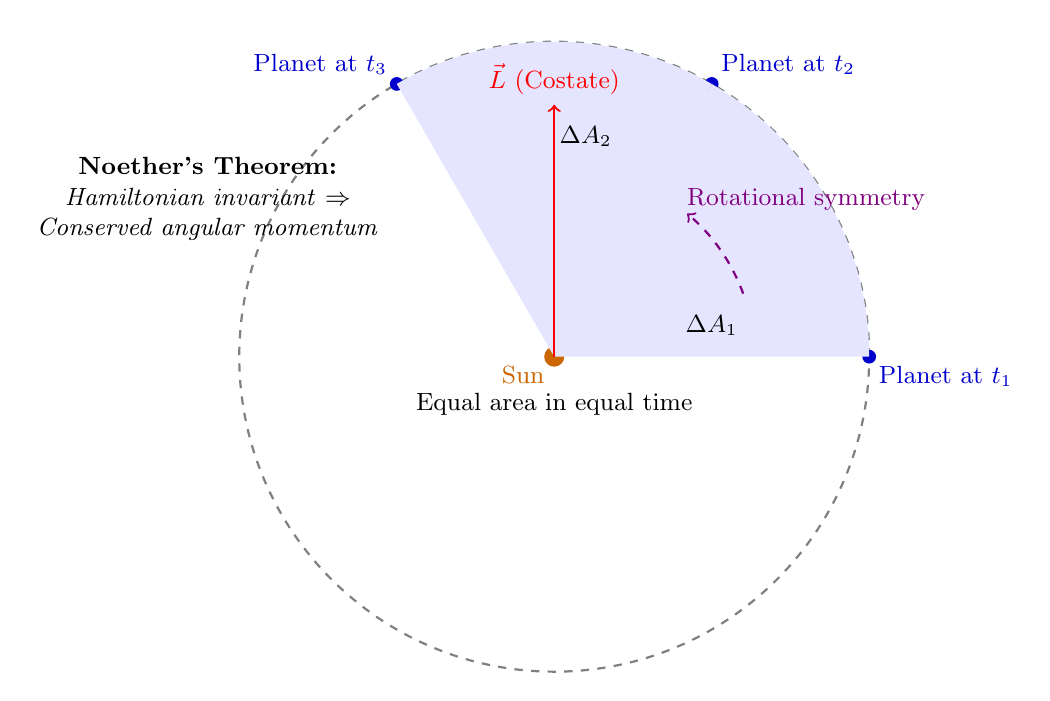
\begin{tikzpicture}[scale=4, every node/.style={font=\small}]
    % Sun
    \filldraw[orange!80!black] (0,0) circle (0.03) node[below left] {Sun};

    % Orbit path
    \draw[gray, thick, dashed] (0,0) circle (1);

    % Planet positions
    \coordinate (P1) at (1,0);
    \coordinate (P2) at ({cos(60)},{sin(60)});
    \coordinate (P3) at ({cos(120)},{sin(120)});
    
    \filldraw[blue!80!black] (P1) circle (0.02) node[below right] {Planet at $t_1$};
    \filldraw[blue!80!black] (P2) circle (0.02) node[above right] {Planet at $t_2$};
    \filldraw[blue!80!black] (P3) circle (0.02) node[above left] {Planet at $t_3$};

    % Swept areas (two sectors)
    \fill[blue!10] (0,0) -- (P1) arc (0:60:1) -- cycle;
    \fill[blue!10] (0,0) -- (P2) arc (60:120:1) -- cycle;

    % Angular momentum vector
    \draw[->, thick, red] (0,0) -- (0,0.8) node[above] {$\vec{L}$ (Costate)};

    % Equal area labels
    \node at (0.5,0.1) {$\Delta A_1$};
    \node at (0.1,0.7) {$\Delta A_2$};
    \node at (0.0,-0.15) {Equal area in equal time};

    % Rotational symmetry arc
    \draw[->, thick, violet, dashed] (0.6,0.2) arc (20:50:0.6);
    \node[violet] at (0.8,0.5) {Rotational symmetry};

    % Hamiltonian symmetry note
    \node[align=center] at (-1.1,0.5) {
        \textbf{Noether’s Theorem:}\\
        \textit{Hamiltonian invariant} $\Rightarrow$\\
        \textit{Conserved angular momentum}
    };

\end{tikzpicture}
\caption{Kepler’s Second Law interpreted through control theory: the conservation of angular momentum as a costate, the rotational symmetry of the Hamiltonian, and equal areas swept out in equal times.}
\end{figure}

\begin{table}[H]
\vspace{1.5em} % Space above the table
\centering
\renewcommand{\arraystretch}{2.0} % Even more row height
\begin{tabular}{>{\raggedright\arraybackslash}p{0.45\linewidth} | >{\raggedright\arraybackslash}p{0.45\linewidth}}
\toprule
\addlinespace[1.2em]
\textbf{Classical Newtonian Mechanics} & \textbf{Optimal Control Theory (Pontryagin)} \\
\addlinespace[1.2em]
\midrule
\addlinespace[1.2em]

\textbf{Framework:} Newton's laws, force-based dynamics &
\textbf{Framework:} Pontryagin's Maximum Principle, costate dynamics \\
\addlinespace[1.2em]

Gravitational force is central: $\vec{F} = -\frac{GMm}{r^2} \hat{r}$ &
Hamiltonian $H(x, \lambda)$ is invariant under rotation \\
\addlinespace[1.2em]

Zero torque: $\vec{\tau} = \vec{r} \times \vec{F} = 0$ &
By Noether’s theorem, symmetry $\Rightarrow$ conserved quantity \\
\addlinespace[1.2em]

Conservation of angular momentum: $\vec{L} = \vec{r} \times \vec{p}$ &
Conservation of costate: $\lambda_\theta = \text{const}$ (angular momentum as costate) \\
\addlinespace[1.2em]

Area swept: $\frac{dA}{dt} = \frac{1}{2} r^2 \frac{d\theta}{dt}$ &
Costate conservation implies $\frac{dA}{dt} = \text{const}$ \\
\addlinespace[1.2em]

\textit{Equal areas in equal times} is a geometric result &
\textit{Equal areas in equal times} is a necessary condition for optimality \\
\addlinespace[1.2em]

\textbf{Conclusion:} Result of torque-free motion under a central force &
\textbf{Conclusion:} A structural constraint from rotational symmetry in Hamiltonian \\
\addlinespace[1.2em]
\bottomrule
\end{tabular}
\vspace{1.5em} % Space below the table
\caption{Comparison of Kepler’s Second Law under classical mechanics and optimal control theory. Both yield conservation of angular momentum, but through distinct interpretive frameworks.}
\end{table}




\subsection{The Philosophy of Trajectories: An Imagined Soviet Debate}

When I picture the development of optimal control theory in the Soviet Union, I don’t just imagine engineers hunched over missile paths. I imagine something more ideological—a scene in which the foundations of classical physics itself are called into question. After all, Newtonian mechanics wasn’t just math; it was metaphysics. It treated the universe like a passive machine, unfolding from divine initial conditions. That might fly in Cambridge, but in Moscow? In the middle of the 20\textsuperscript{th} century? Not without a dialectical audit.

So here’s how I imagine things going down, somewhere inside a smoky academic office at the Academy of Sciences, circa 1957:

{
\ttfamily
\textbf{Party Official:} Comrade Pontryagin, I’ve been reviewing the foundations of your optimal control theory.  

\textbf{Pontryagin:} Yes, it’s all based on the Hamiltonian formalism. Very effective for guiding dynamic systems toward—  

\textbf{Party Official:} Hamiltonian, yes. Newtonian, Lagrangian, all very... tsarist-sounding.  

\textbf{Pontryagin:} I assure you, there’s nothing religious in the equations.  

\textbf{Party Official:} Are you aware that Newton said, “The most beautiful system of the sun, planets, and comets could only proceed from the counsel and dominion of an intelligent and powerful being”?  

\textbf{Pontryagin:} Perhaps... but it models ballistic motion quite reliably.  

\textbf{Party Official:} And what of Lagrange, who wrote that the goal of mechanics is to “glorify the works of the Creator through the elegance of mathematical expression”? Or Hamilton, who referred to dynamics as “a science of the divine harmonies of motion”?  

\textbf{Pontryagin:} Yes, well... I mostly skipped the theological prefaces.  

\textbf{Party Official:} It’s not about prefaces. It’s about foundations. These men built mechanics on top their religious beliefs. We need a framework grounded in dialectical materialism... not theology.  

\textbf{Pontryagin:} You want a dialectical Hamiltonian?  

\textbf{Party Official:} I want mathematics rooted in material reality, not metaphysical abstraction. Marx didn’t optimize over cotangent bundles. He studied systems in contradiction.  

\textbf{Pontryagin:} Then let me show you the adjoint equation. It doesn’t just observe: it responds. It evolves with feedback. That’s the costate: a shadow that adapts to the system’s goals.  

\textbf{Party Official:} Now you're talking. Control, feedback, transformation—this is Marxist calculus.  

\textbf{Pontryagin:} So... we keep the equations, just add historical agency?  

\textbf{Party Official:} Precisely. Keep your variational principles. Just make sure they steer us toward socialism. 
}

